\chapter{Captures d'écran}

Ce chapitre présente, à travers des captures d'écran, le fonctionnement réel de l'outil
NetSentry développé durant le stage : tableau de bord, détail d'un appareil, alertes,
historique des scans, ainsi que l'historique de versionnage du projet sur GitHub.

\section{Démonstration}

Les captures d'écran suivantes illustrent le fonctionnement réel de l'outil, à partir
d'un scan effectué sur un réseau local de test : le tableau de bord présente l'ensemble
des appareils détectés avec leur statut, le détail d'un appareil retrace son historique
de détection, la page des alertes signale les appareils non reconnus, et l'historique
des scans conserve la trace de chaque exécution.

\begin{figure}[H]
    \centering
    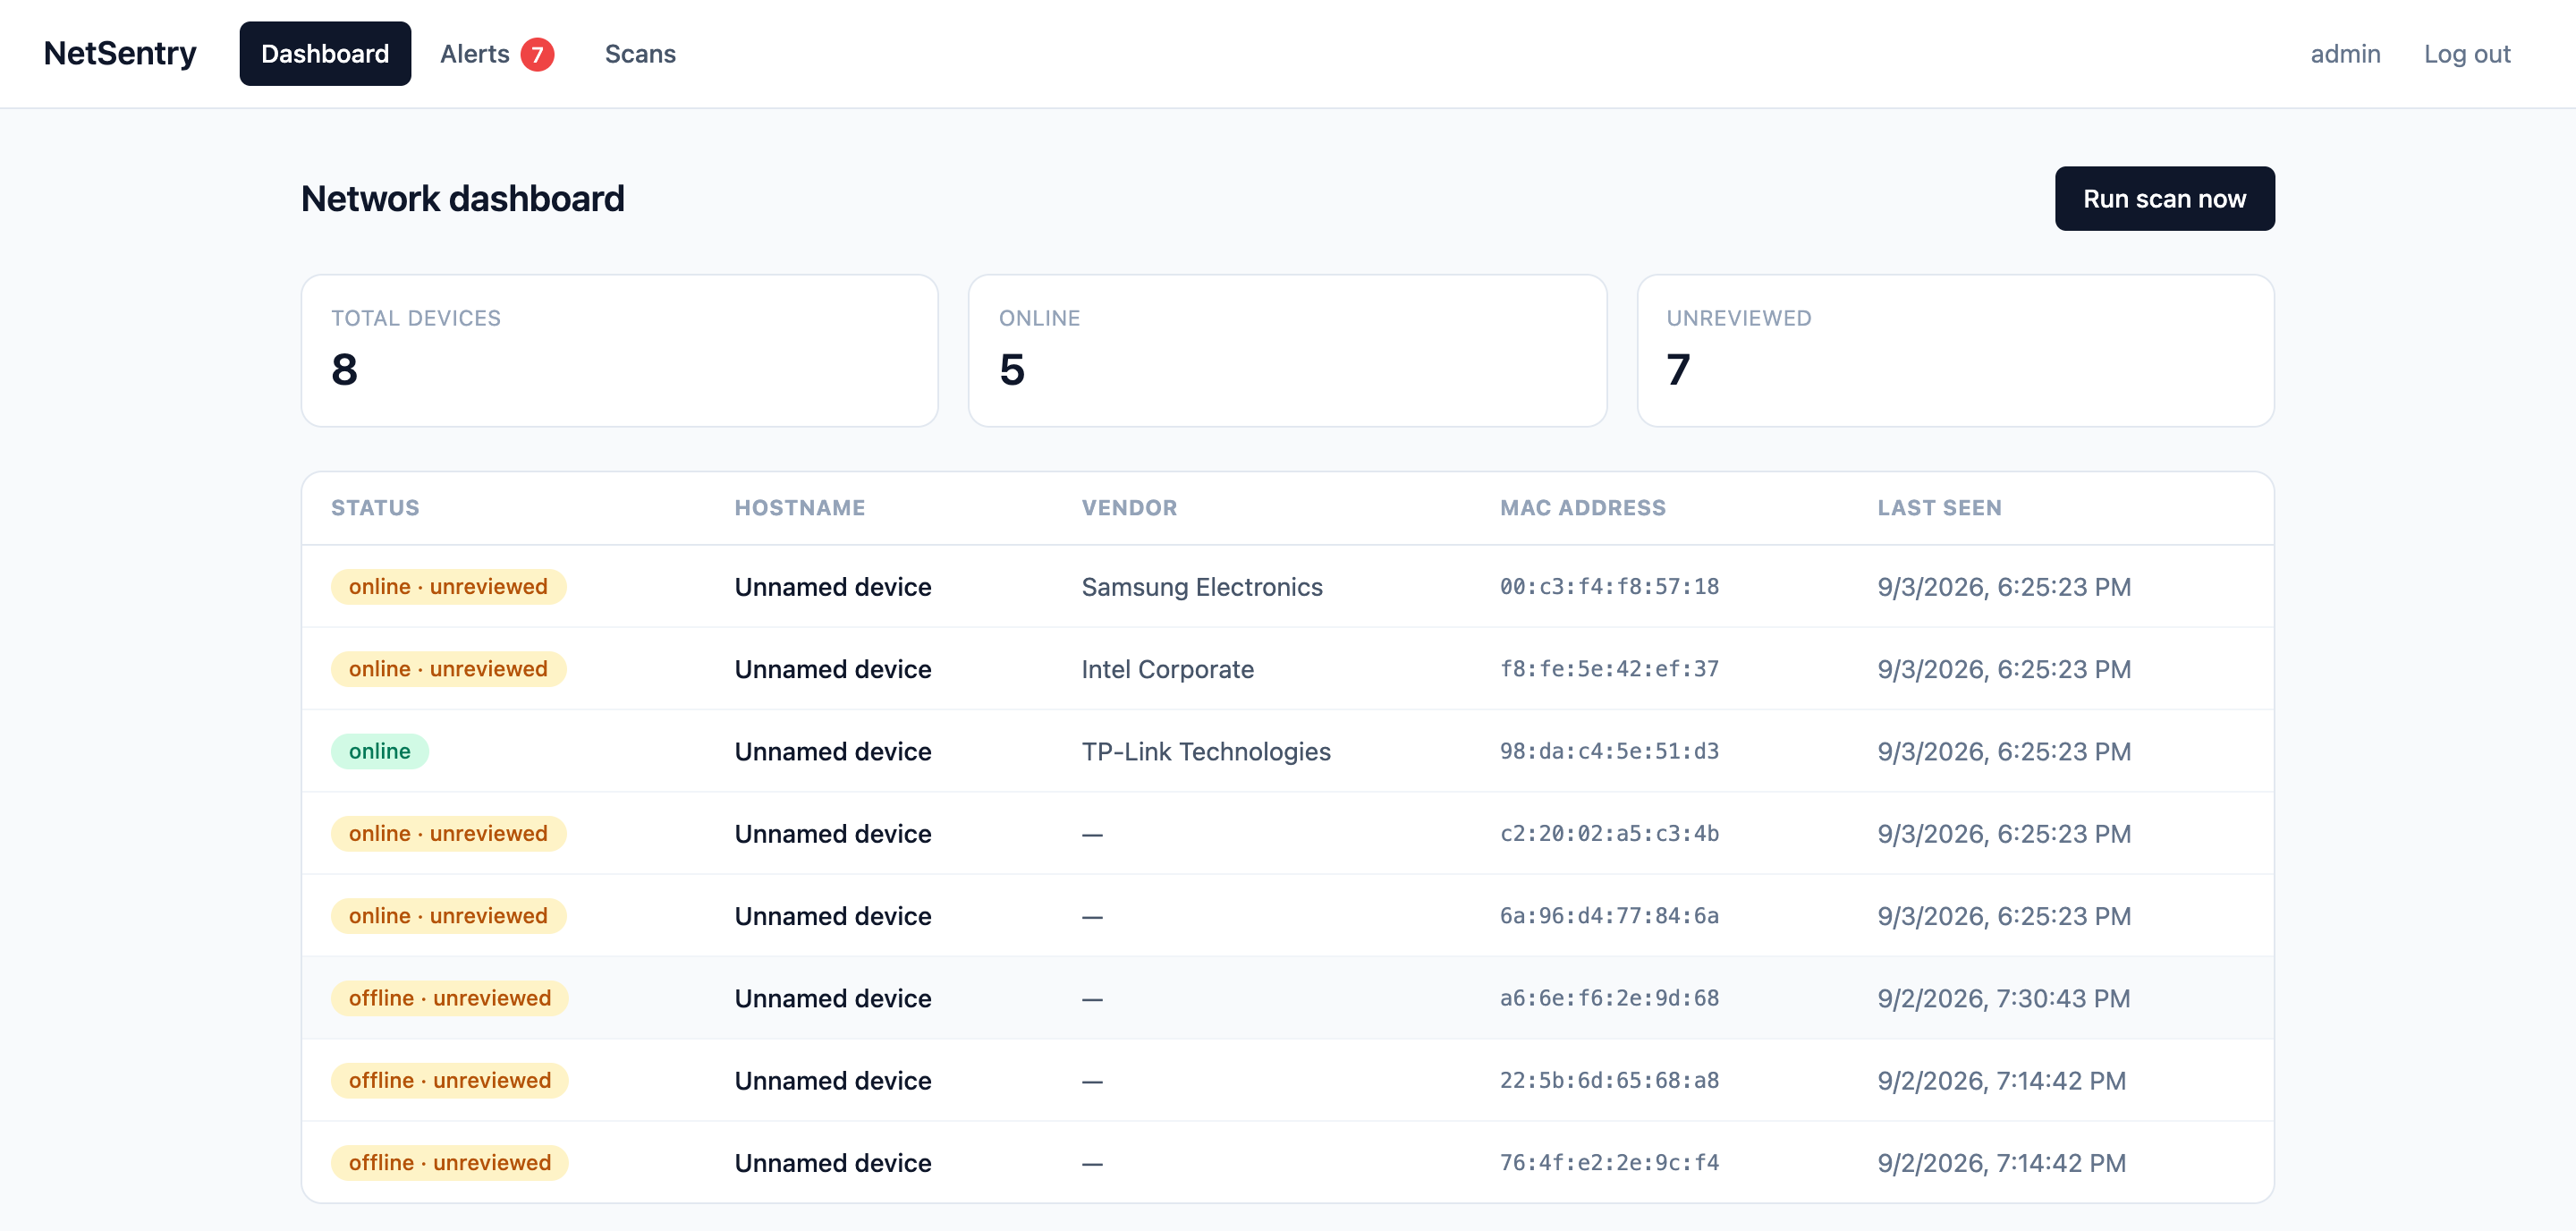
\includegraphics[width=\textwidth]{figures/dashboard.png}
    \caption{Tableau de bord : vue d'ensemble des appareils détectés sur le réseau}
    \label{fig:dashboard}
\end{figure}

\begin{figure}[H]
    \centering
    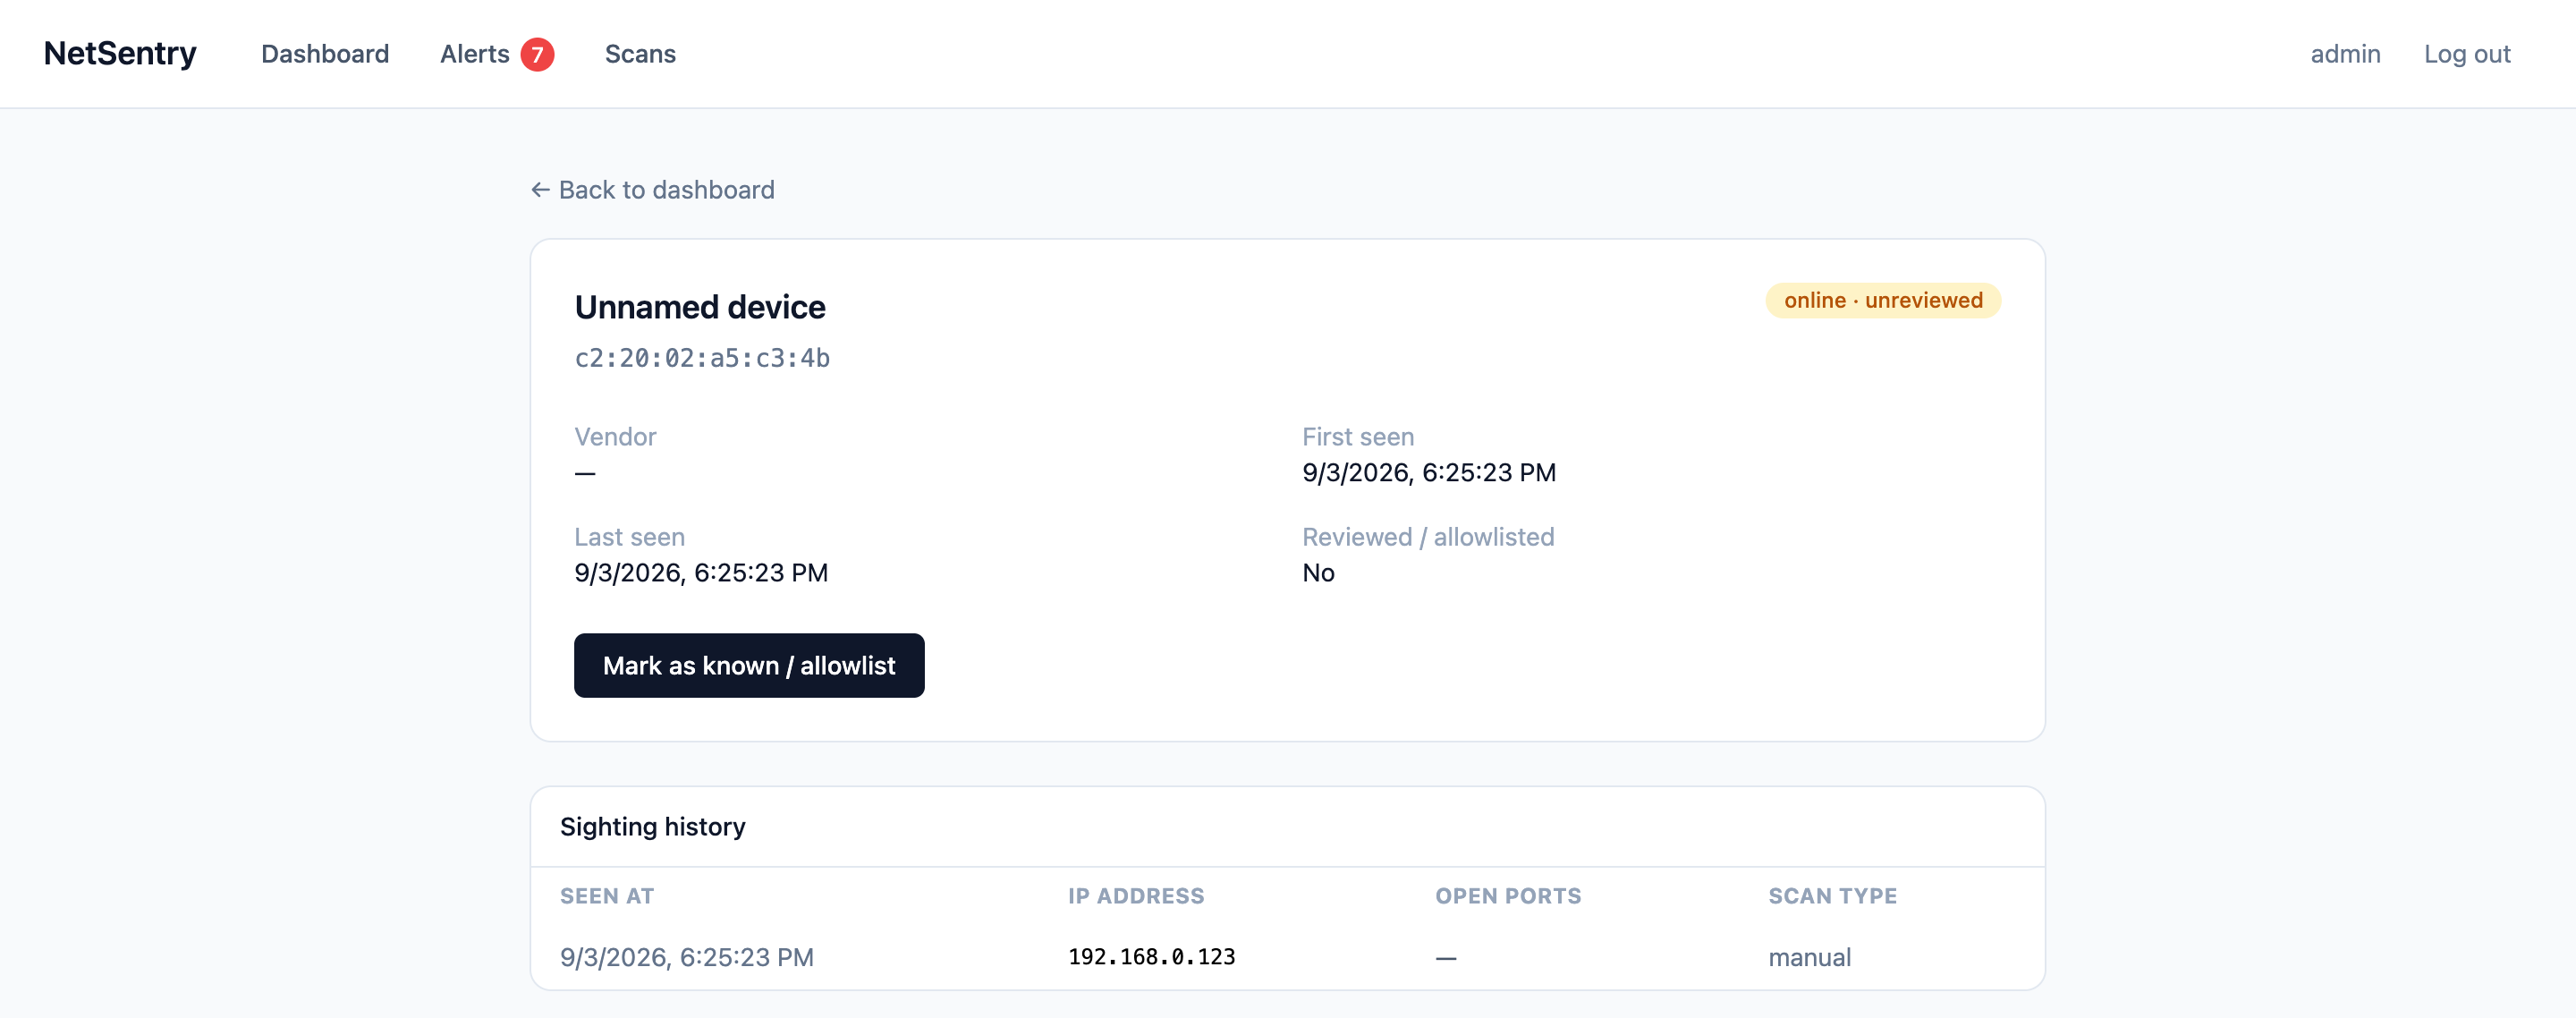
\includegraphics[width=\textwidth]{figures/device_detail.png}
    \caption{Détail d'un appareil : historique de détection et mise en liste blanche}
    \label{fig:device-detail}
\end{figure}

\begin{figure}[H]
    \centering
    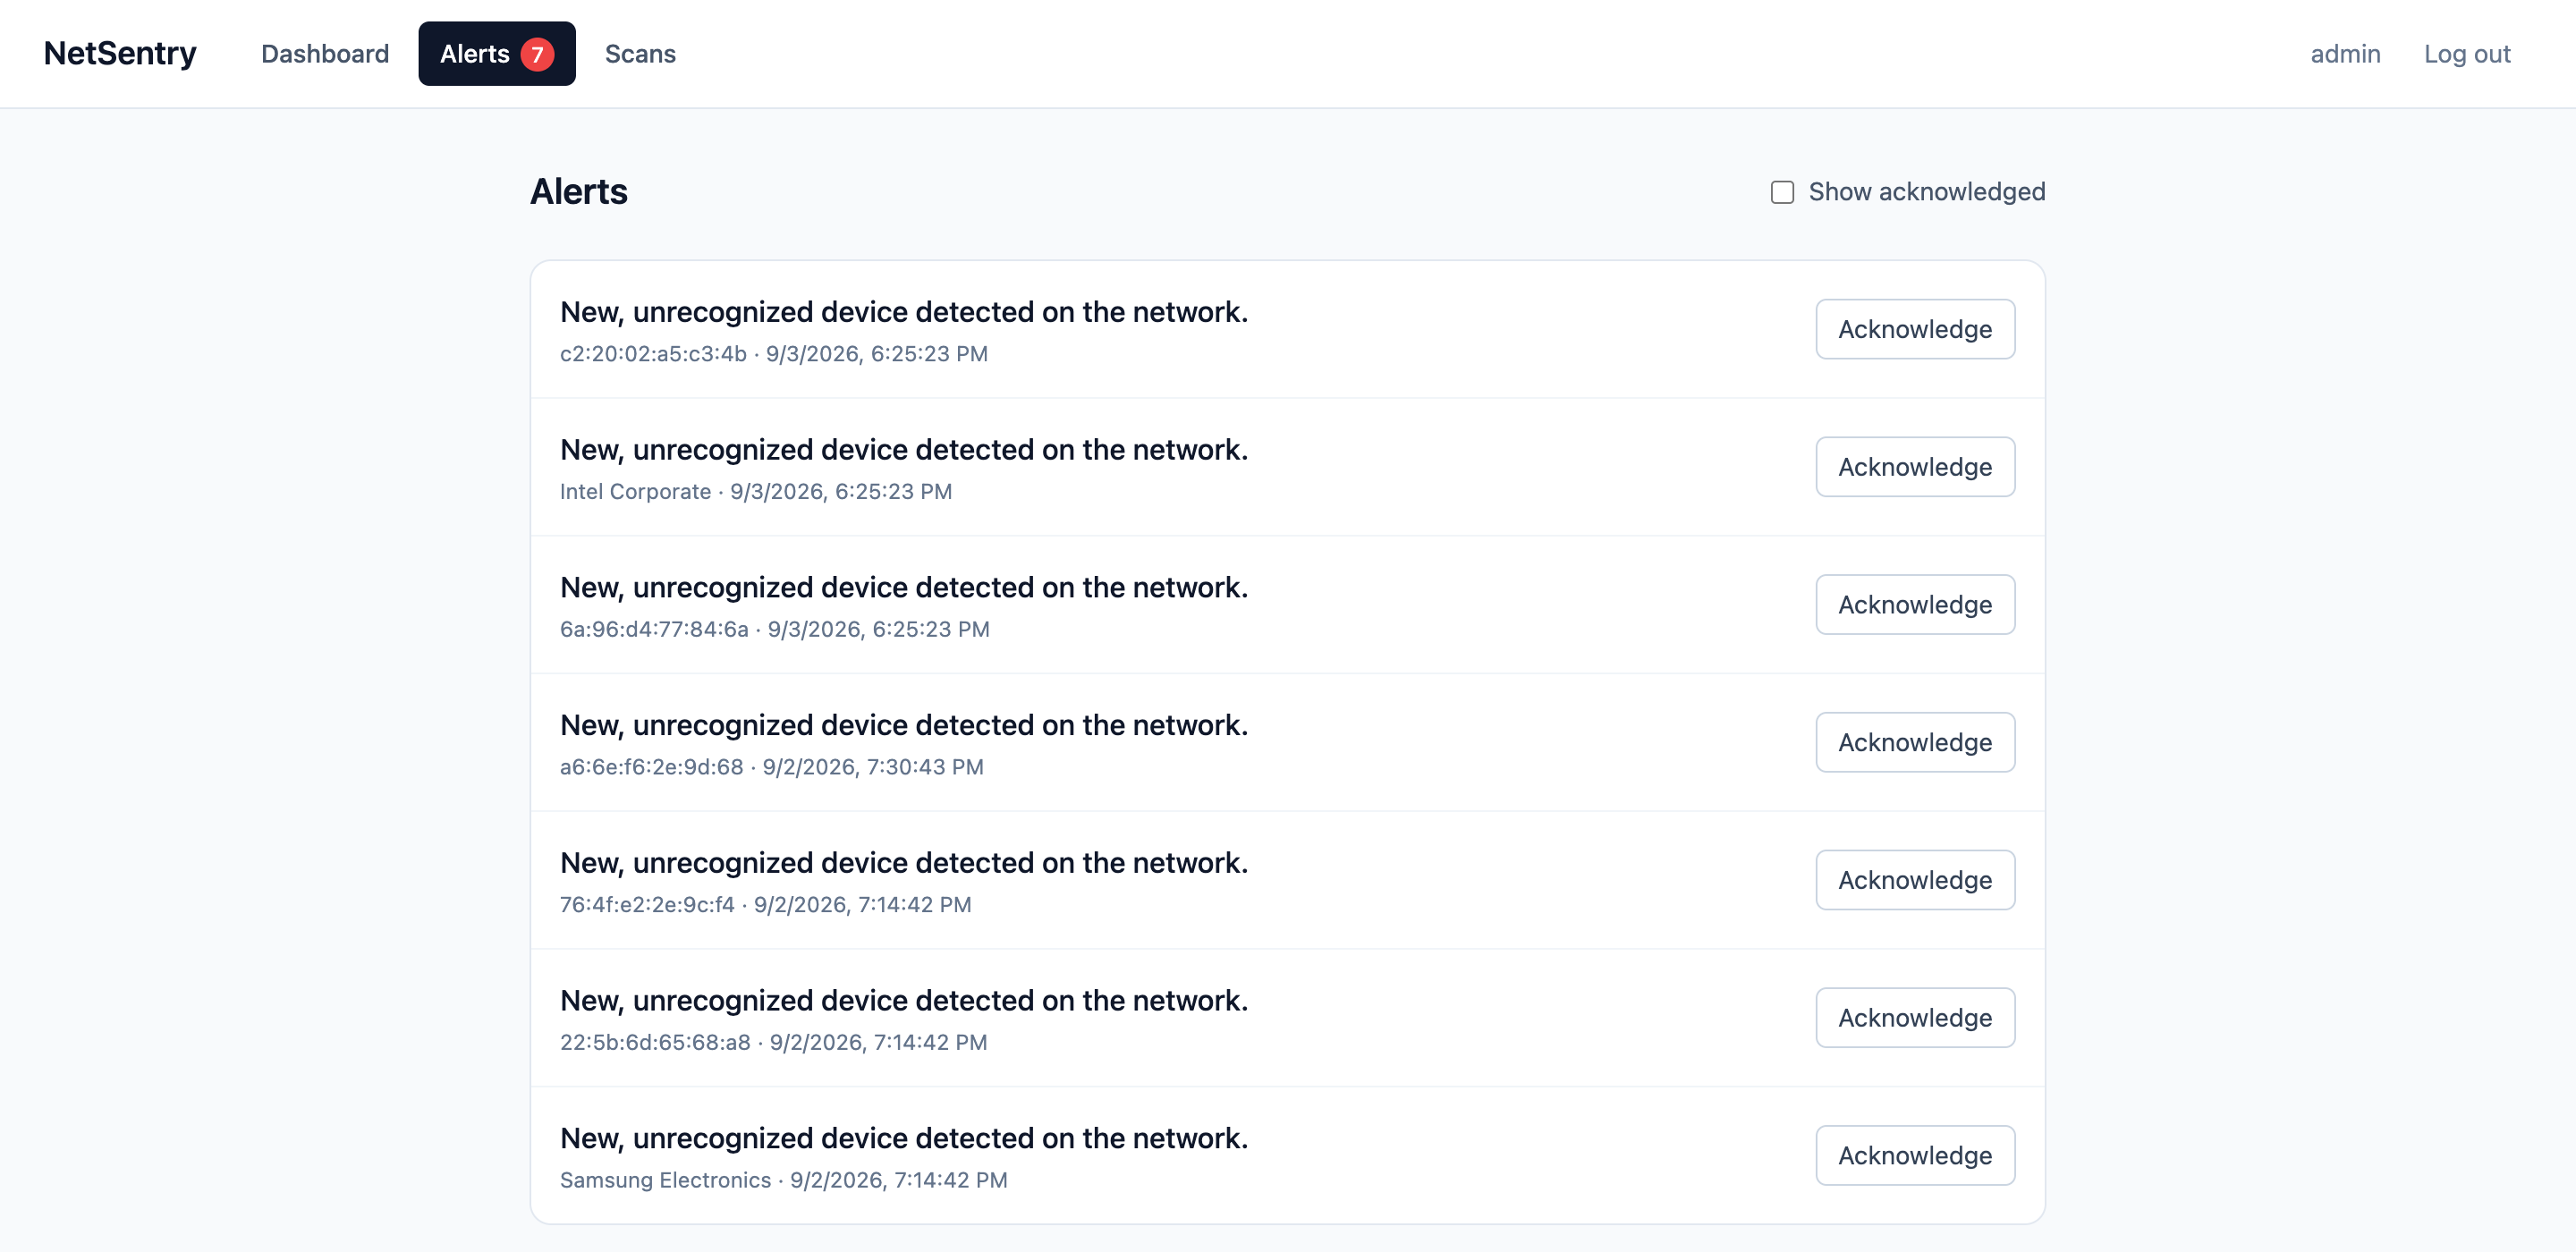
\includegraphics[width=\textwidth]{figures/alerts.png}
    \caption{Alertes : appareils non reconnus signalés après un scan}
    \label{fig:alerts}
\end{figure}

\begin{figure}[H]
    \centering
    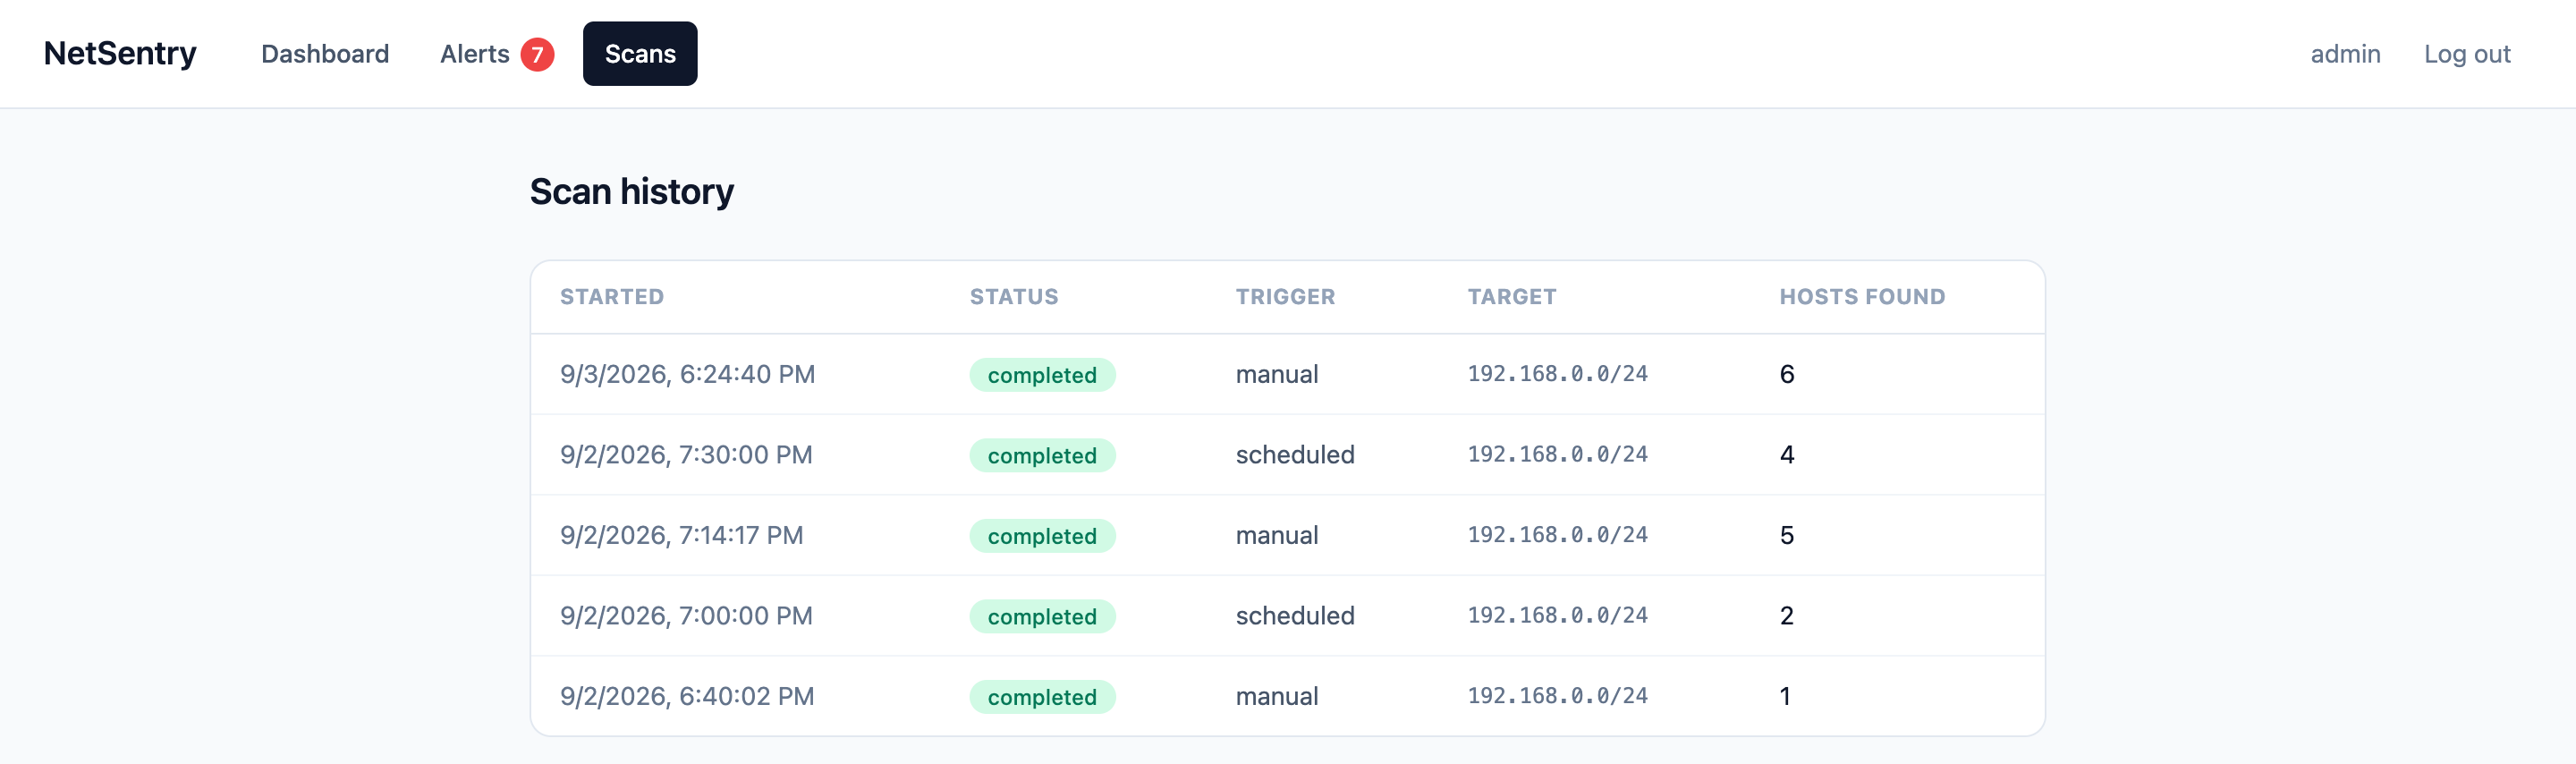
\includegraphics[width=\textwidth]{figures/scan_history.png}
    \caption{Historique des scans exécutés (manuels et planifiés)}
    \label{fig:scan-history}
\end{figure}

\section{Versionnage}

Le projet est versionné avec Git et hébergé sur un dépôt GitHub public. L'historique
reste volontairement synthétique à ce stade du stage : un commit initial, l'ajout des
documents de cadrage, puis un commit unique regroupant la construction du MVP (backend,
frontend, conteneurisation). Il sera affiné par des commits plus granulaires au fil des
prochaines itérations.

\begin{figure}[H]
    \centering
    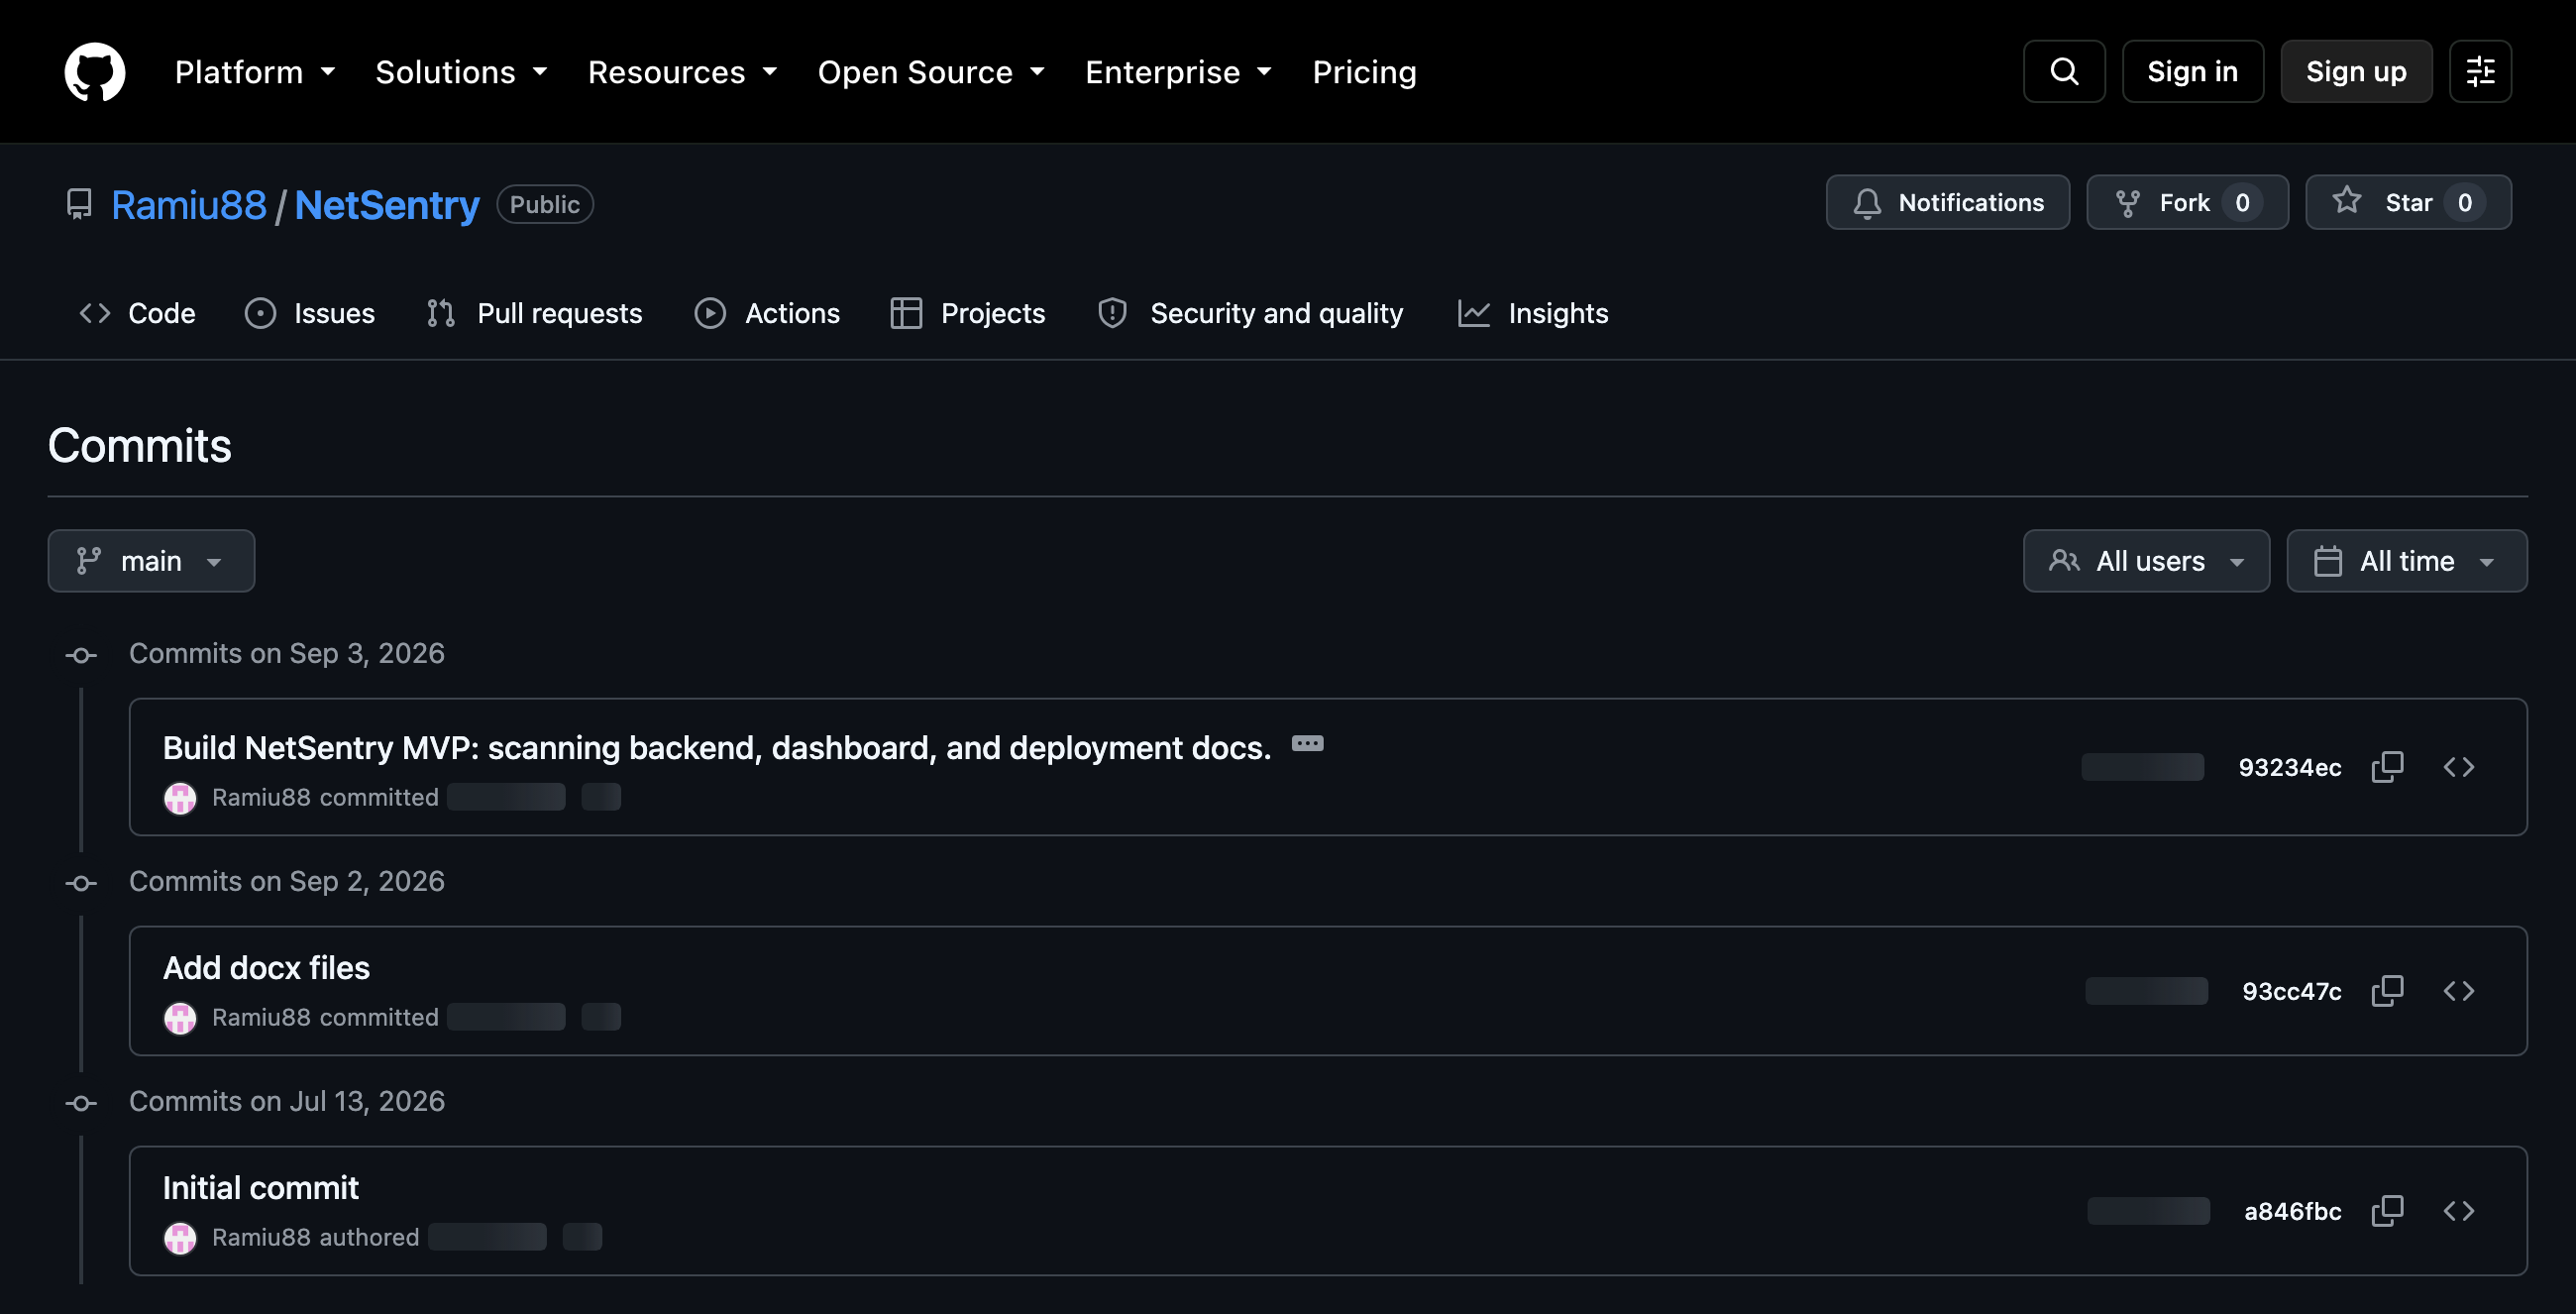
\includegraphics[width=\textwidth]{figures/github_commits.png}
    \caption{Historique des commits du dépôt GitHub NetSentry}
    \label{fig:github-commits}
\end{figure}
